\documentclass[]{article}
\usepackage[T1]{fontenc}
\usepackage[top=1in, bottom=1in, left=1in, right=1in]{geometry}
\usepackage{commath,amsmath,amssymb,amsfonts}
\usepackage{newtxtext, newtxmath}
\usepackage{float}
\usepackage{algorithmic}
\usepackage{graphicx}
\graphicspath{{./images/}}
\usepackage{textcomp}
\usepackage{xcolor}
\usepackage[backend=biber, sorting=none]{biblatex}
\usepackage[hidelinks]{hyperref}

%uncomment below line to use reference file
\addbibresource{references.bib}

%opening
\title{VR Report}
\author{Benjamin Russell - fdmw97}
\date{}

\begin{document}

\maketitle

\section{Static Renders}
Presented below are static renders demonstrating the inverse Lateral Chromatic Aberration (LCA) correction, fragment shader based pre-distortion, and mesh based pre-distortion.
\begin{figure}[h!]
	\centering
	\begin{minipage}[H]{0.2\textwidth}
		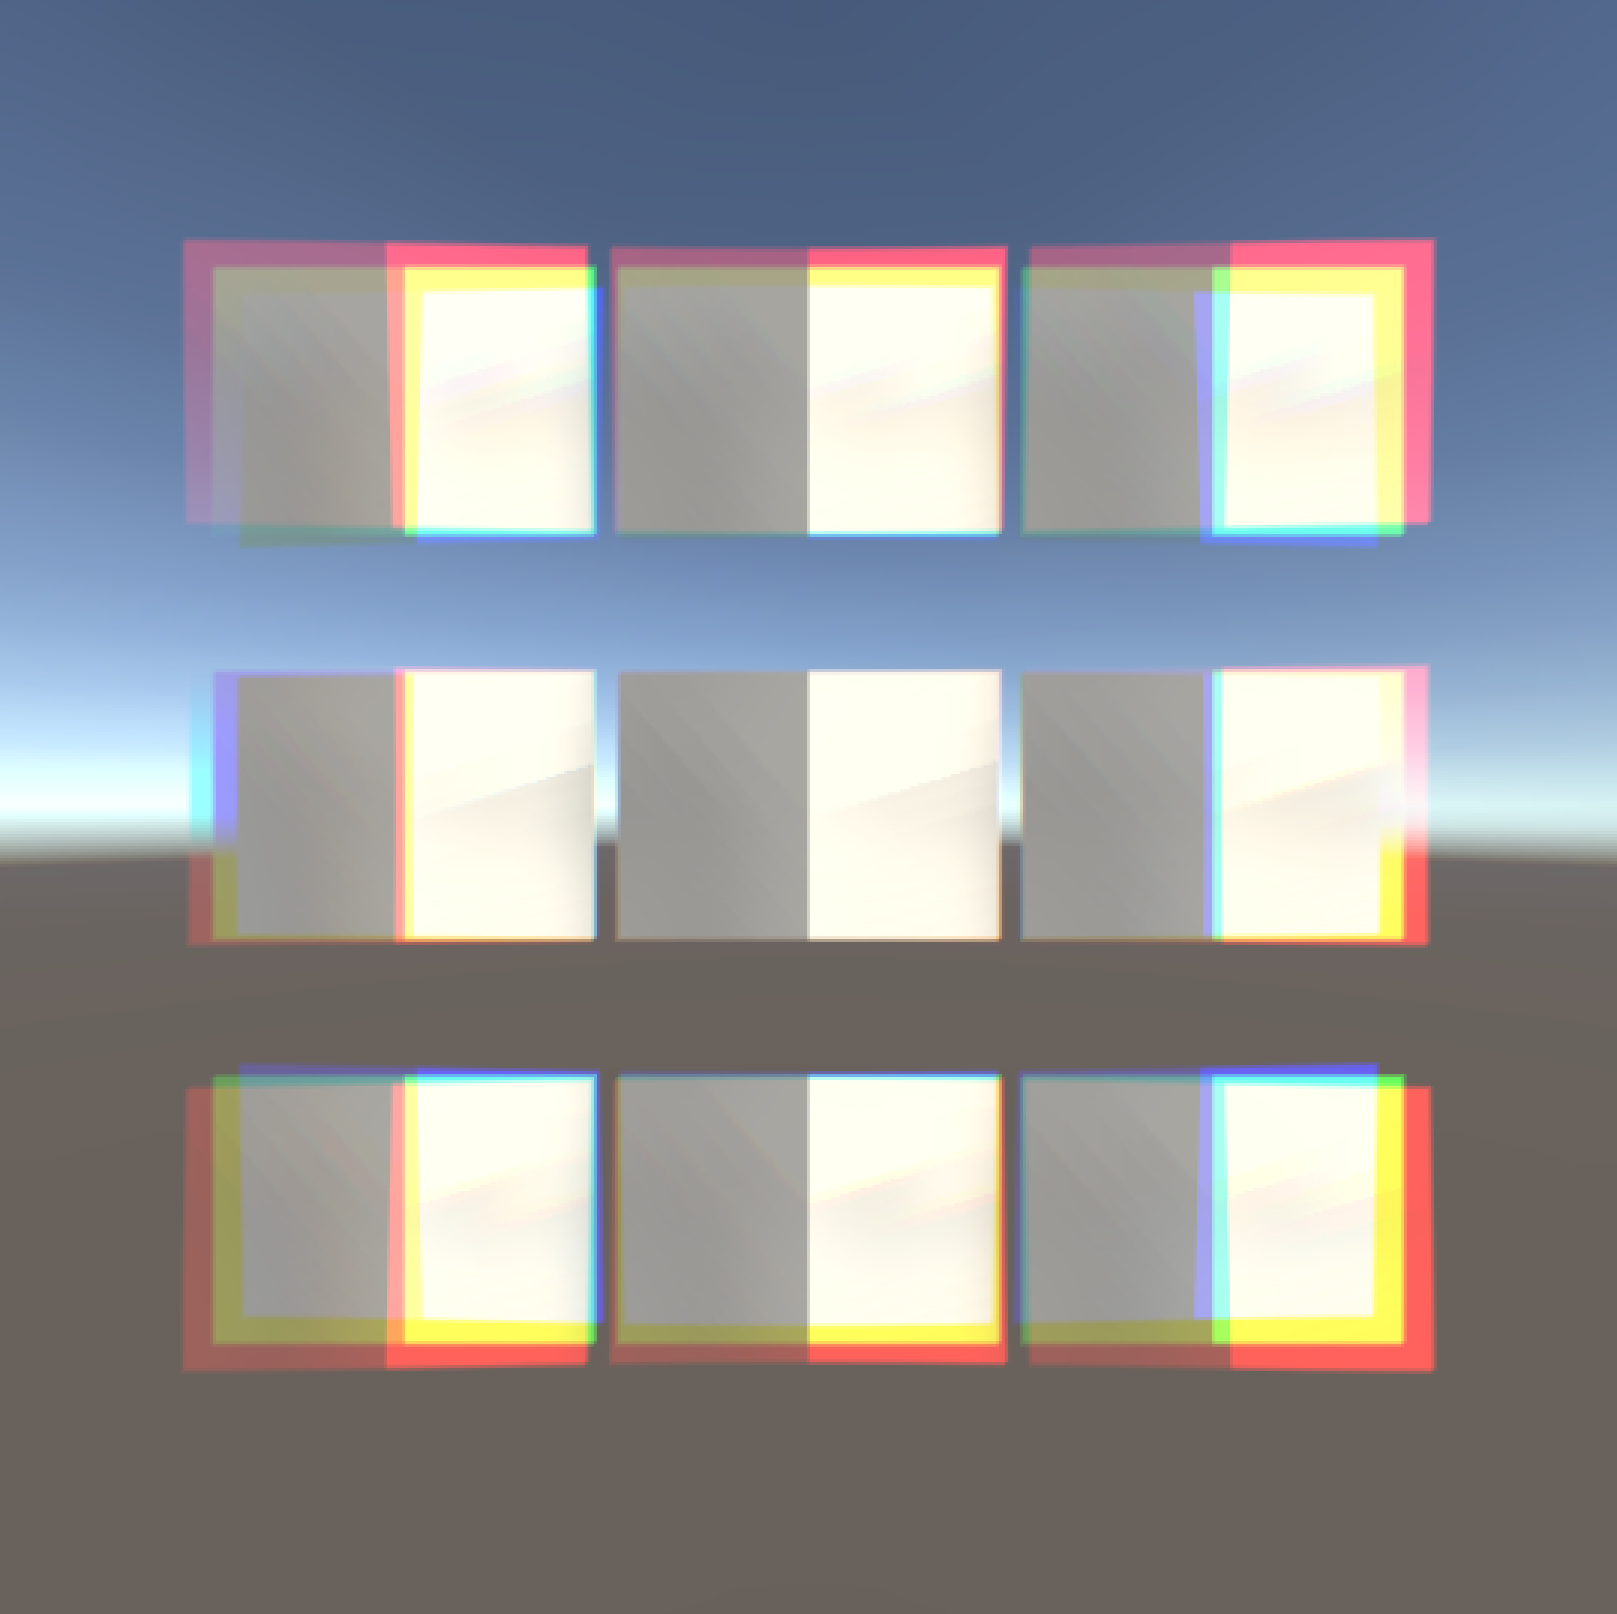
\includegraphics[width=4cm]{LCA_45}
		\caption{Static render of cubes at 45 degrees using inverse LCA correction}
		\label{fig:lca_45}
	\end{minipage}
	\hfill
	\begin{minipage}[H]{0.2\textwidth}
		
\includegraphics[width=4cm]{Barrel_Frag_45}
		\caption{Static render of cubes at 45 degrees using fragment shader based pre-distortion}
		\label{fig:frag_45}
	\end{minipage}
	\hfill
	\begin{minipage}[H!]{0.2\textwidth}
		
\includegraphics[width=4cm]{Barrel_Vec_45}
		\caption{Static render of cubes at 45 degrees using mesh based pre-distortion with 512 triangle mesh}
		\label{fig:vec_45}
	\end{minipage}
\end{figure}

\section{Comparison of Pixel and Mesh Based Pre-Distortion}
Pixel based pre-distortion has the advantage of being much easier to implement that mesh based pre-distortion as it is simply sampling each pixel from the texture at its new distorted radius. When compared to a mesh based method with a low vertex/triangle count the pixel based method produces far more accurate results as the accuracy is as good as the textures resolution which can be made very high quite easily. This is shown in \autoref{fig:res_mesh_comp} where it is clear that the since the texture/frame-buffer resolution is greater than the vertex/triangle count of the mesh the pixel based pre-distortion is more accurate, with the low vertex mesh based method showing hard edges and other distortions on the outer cubes rather than the smooth curved barrel distorted edges in the pixel based method.
\begin{figure}[H]
	\centering
	\begin{minipage}[H]{0.2\textwidth}
		
\includegraphics[width=4cm]{Barrel_Frag_45}
	\end{minipage}
	\hspace{1cm}
	\begin{minipage}[H]{0.2\textwidth}
		
\includegraphics[width=4cm]{Barrel_Vec_32}
	\end{minipage}
	\caption{Comparison of pixel based pre-distortion 512x512 resolution (left) and mesh based pre-distortion 32 triangle mesh (right)}
	\label{fig:res_mesh_comp}
\end{figure}
The advantage of using a the mesh based method is in the number of required calculations in the shader. When using the pixel based method the distorted radius is calculated on a per pixel basis which in the case of the 512x512 render texture used in this project is 262,144 distortion calculations. When compared to using a mesh of just 128 triangles/81 vertices which only requires distorting the individual vertices so 81 distortion calculations, the actual distortion of the image using the mesh based method leverages the interpolation that takes place between the fragment and vertex shader in order to save on direct computation of distortion for each pixel as these values are interpolated based on the vertex distortions instead. The number of texture lookups in both methods is determined by the output resolution of the scene as we have to sample the texture for each fragment to determine the final colour on the screen. Even though the computational cost is reduced by using the mesh based method to calculate where to sample the texture (thanks to interpolation), it is still necessary to sample the texture for the same number of fragments as the pixel based method.
\subsection{Effect Of Vertex Count On Mesh Based Pre-Distortion}
The number of vertices used for the mesh based method affects the distortion quality such that a low number of vertices produces low quality barrel distortion as there are not many vertices to interpolate texture coordinates between resulting in jagged edges to the distorted image. Using a greater number of vertices allows requires more calculations due to the increased vertex count, however it means the interpolation between each set of vertices more accurately reflects what the distortion should really look like. This is demonstrated in \autoref{fig:vert_comp} with the 25 vertex mesh clearly displaying the jagged edges, the 81 vertex mesh has some minor jagged edges which may be noticeable when using an HMD, and the 289 vertex mesh has the smoothest edges however the increase in vertex count does have diminishing returns. The increase vertex count also had a small affect on the frames per second (FPS) rendered and the time taken for the camera to render the scene, such that with a 25 vertex mesh rendering the scene took around 1.5ms whereas using the 289 vertex mesh increased that to around 4.7ms. This increase is hardly noticeable when watching the cubes rotate and made not perceivable difference to the observed FPS.
\begin{figure}[H]
	\centering
	\begin{minipage}[H]{0.2\textwidth}
		
\includegraphics[width=4cm]{Barrel_Vec_32}
	\end{minipage}
	\hfill
	\begin{minipage}[H]{0.2\textwidth}
		
\includegraphics[width=4cm]{Barrel_Vec_128}
	\end{minipage}
	\hfill
	\begin{minipage}[H]{0.2\textwidth}
		
\includegraphics[width=4cm]{Barrel_Vec_45}
	\end{minipage}
	\caption{Static render using 25 vertex mesh (left), 81 vertex mesh (middle), and 289 vertex mesh (right)}
	\label{fig:vert_comp}
\end{figure}
\subsection{Modelling The Lens}
As is standard practice the pre-distortion was performed using and inverse distortion function, and the lens using the forward distortion function, given below:
\begin{gather*}
	r_d = f(r_u) = r_u + c_1r_u^3+c_2r_u^5 \\
	f^{-1}(r_d) = r_d - r_d\left(
	\frac{c_1r_d^2+c_2r_d^4+c_1^2r_d^4+c_2^2r_d^8+2c_1c_2r_d^6}{1+4c_1r_d^2+6c_2r_d^4}
	\right)
\end{gather*}
Where $r$ is a points radius in polar coordinates, and $c_1$, $c_2$ are constants. This choice of inverse uses the inverse given in the brief as part of it, and was chosen based on~\cite{inverse}. \autoref{fig:inv_comp} shows that when using the given inverse function when simulating the lens the result is just a zoomed in version of the pre-distortion, whereas when using the function given in~\cite{inverse} the result of simulating the lens is almost indistinguishable from the undistorted scene. The slight errors are caused by the interpolation between vertices in the pre-distortion and the lens simulation.
\begin{figure}[H]
	\centering
	\begin{minipage}[H]{0.2\textwidth}
		
\includegraphics[width=4cm]{inv_fail}
	\end{minipage}
	\hspace{1cm}
	\begin{minipage}[H]{0.2\textwidth}
		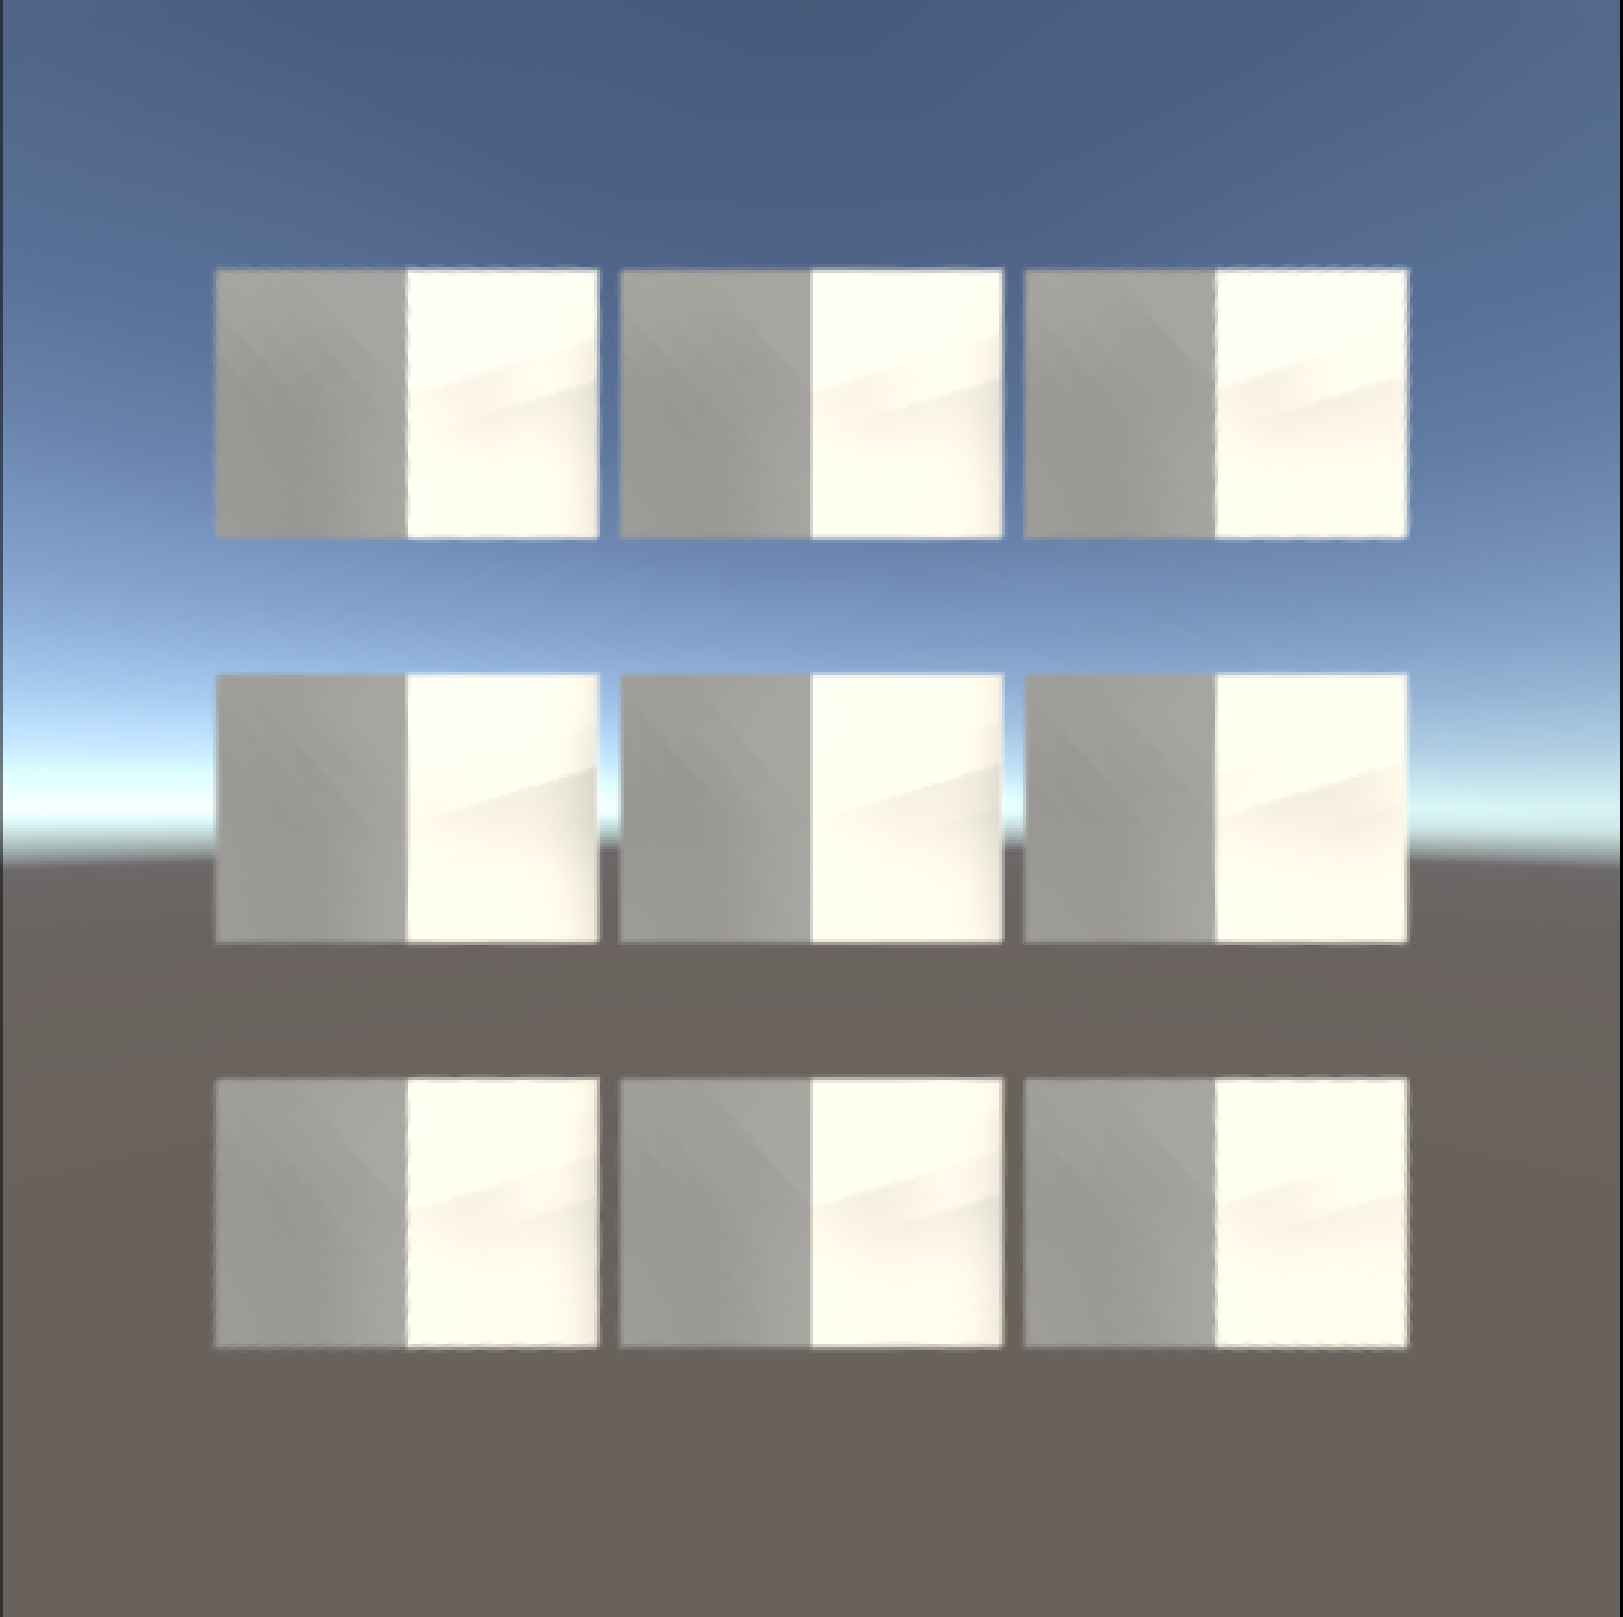
\includegraphics[width=4cm]{inv_success}
	\end{minipage}
	\caption{Comparison of chosen inverse function (right) and function given in the brief (left)}
	\label{fig:inv_comp}
\end{figure}

\autoref{fig:lens_comp} shows that when using the mesh based method the vertex count has has an affect on how the final image will look to the user when passing through the lens after pre-distortion. It is clear that the higher vertex count mesh produces and more accurate final image than the other 2 vertex counts, almost as accurate as the more expensive pixel based method.

\begin{figure}[H]
	\centering
	\begin{minipage}[H]{0.2\textwidth}
		
\includegraphics[width=4cm]{Inv_Vec_32}
	\end{minipage}
	\hfill
	\begin{minipage}[H]{0.2\textwidth}
		
\includegraphics[width=4cm]{Inv_Vec_128}
	\end{minipage}
	\hfill
	\begin{minipage}[H]{0.2\textwidth}
		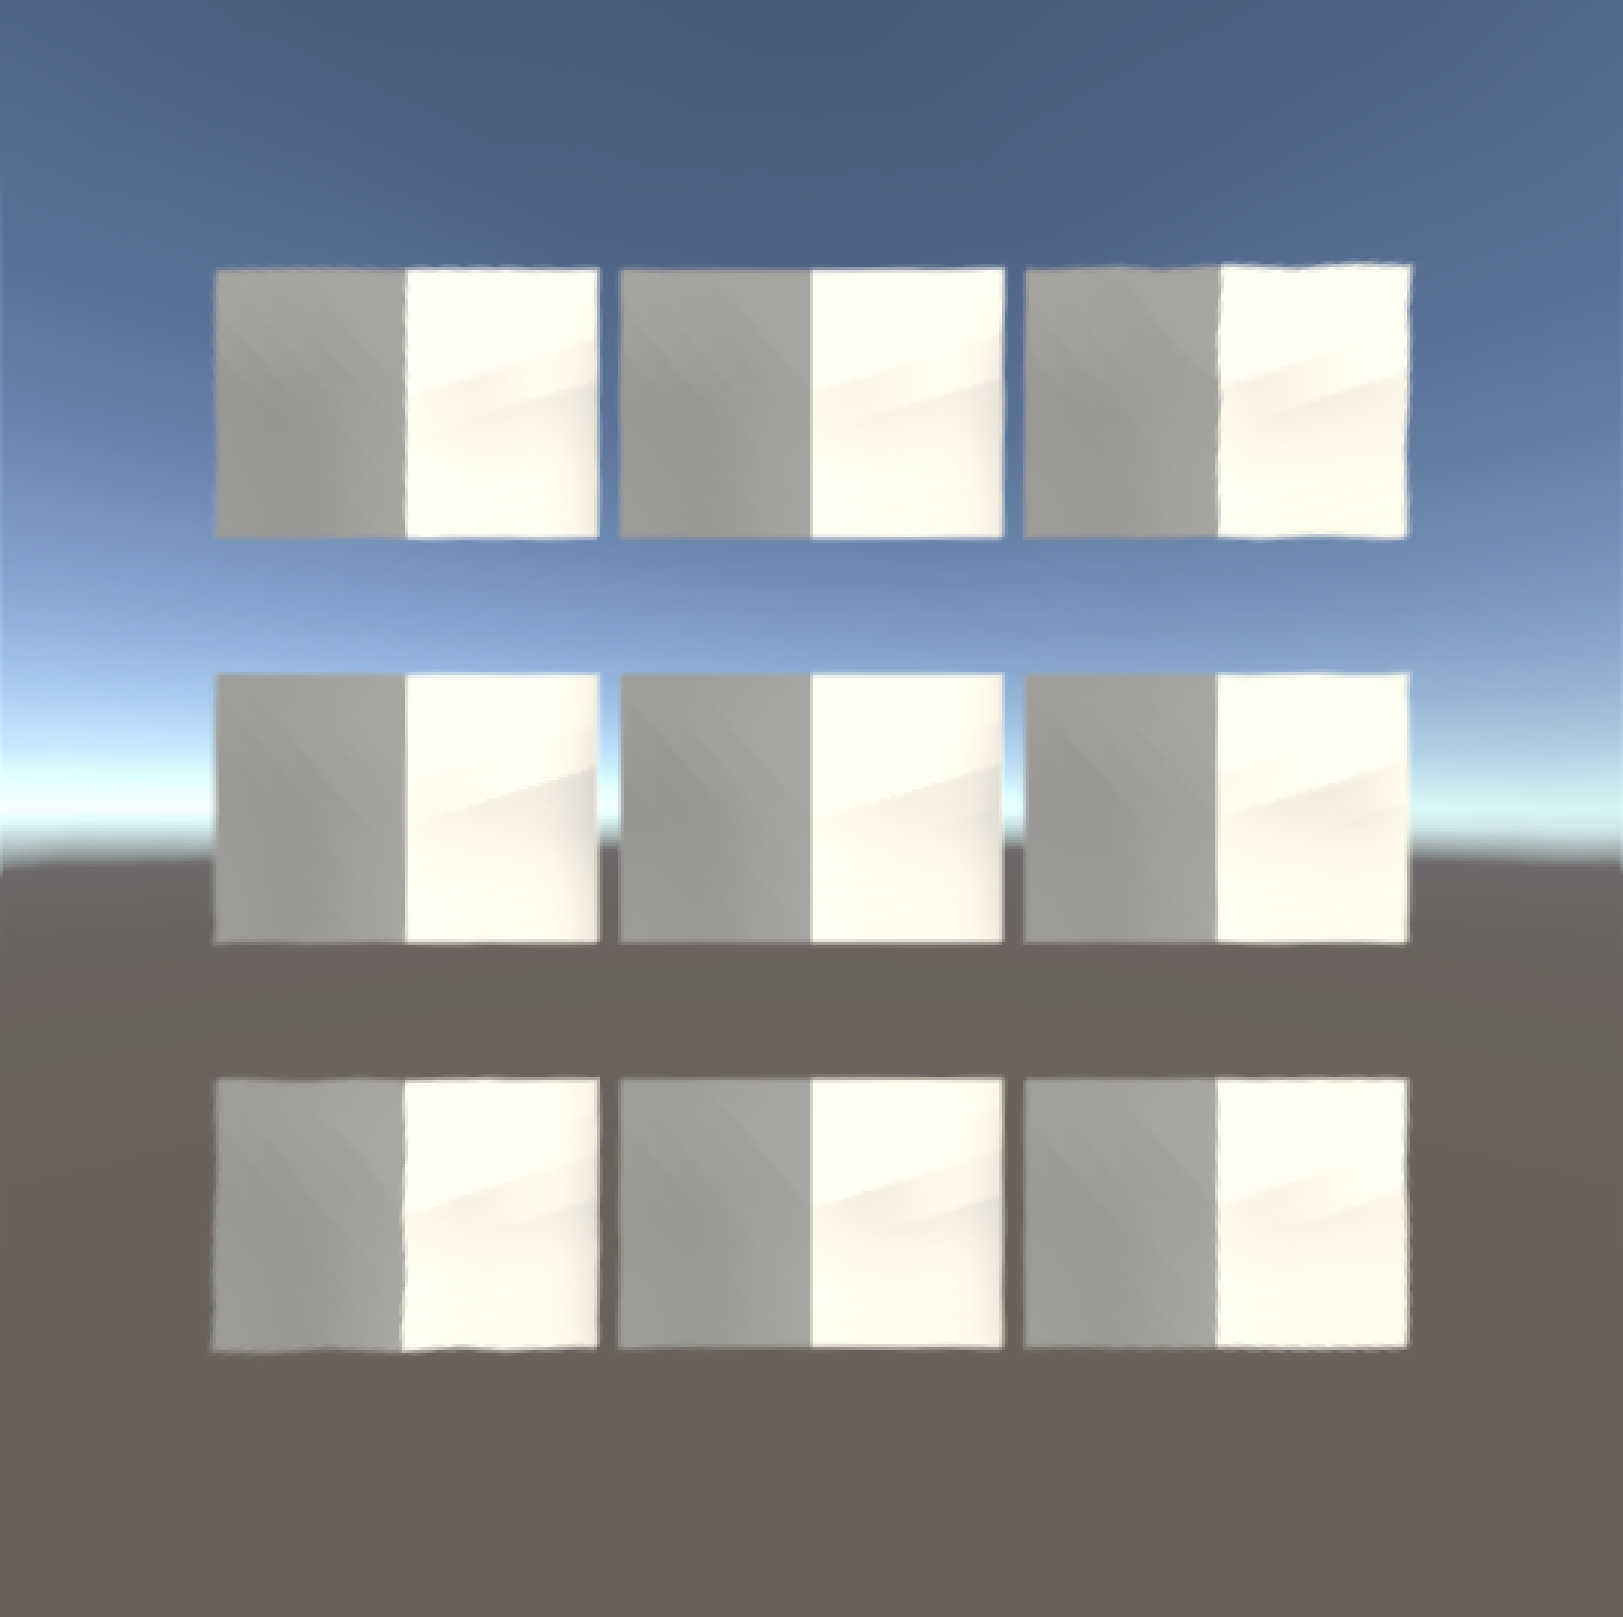
\includegraphics[width=4cm]{Inv_Vec_512}
	\end{minipage}
	\caption{Simulated full pass through the lens using using 25 vertex mesh (left), 81 vertex mesh (middle), and 289 vertex mesh (right)}
	\label{fig:lens_comp}
\end{figure}
\section{The Potential Use of Eye Tracking}
The distortions addressed in this paper are radial distortions based on how a lens acts when light passes through it. For this reason eye tracking would be very helpful for the pre-distortions used. This is because in the current implementation the correction assumes you are constantly looking straight ahead at the very centre of the lens i.e. on-axis. However in a real world scenario a use could be looking off-axis, if this is the case then the optical distortion and chromatic aberration will be much more severe. Therefore eye tracking could be used and a more advanced software based distortion correction method could be used based on the eye tracking to pre-distort based on where the users eyes are actually looking.

\section{Addressing Side-Effects of Pre-Distortion}
The pre-correction performs barrel distortion on a render texture. This results in the edges of the image being squashed and having a reduced resolution, this can mean some loss of detail. The centre of the image can become stretched this can exacerbate aliasing problems that already exist due to the low resolution of most HMDs. Possible solutions to this could be to use an anti-aliasing method such as FXAA or MSAA to remove some of jagged edges from aliasing. The squashing around the edges also means some fragments are calculated that never get drawn to the final frame-buffer using multi-resolution shading to split the scene into separate viewports with the viewports near the edges scaled down to save rendering time.

I would suggest rendering the image at a much greater resolution than the HMDs due to the aforementioned aliasing, as this would allow the use of supersampling anti-aliasing (SSAA). SSAA is the use of the higher resolution image to calculate the correct pixel colours in the downsampled image on the HMD screen in such a way that aliasing can be corrected.

After performing all the corrections e.g. LCA and pre-distortion, the apparent resolution of the final scene will be reduced. This is due to the use of render textures of a fixed resolution at each stage of the pre-distortion process, as well as the pre-distortion introducing aliasing, and \autoref{fig:vert_comp} demonstrates the resolution loss around the periphery when using mesh based pre-distortion. Adding to this is the inverse radial transform used for both the LCA and pre-distortion is only an estimate based on empirically obtained constant values, this means after passing through the lens to the users eyes the final scene will be lacking detail due to minor discrepancies between the inverse transform and the actual lens transform. The ramifications on modern headsets is that it may be more worthwhile to pursue hardware solutions such as Fresnel lenses to reduce the initial distortion, or layering a second lens in the headset to perform the pre-distortion rather than using software. These hardware solutions could then be further backed up by software correction based on eye tracking to perform off-axis corrections or foveated rendering so that the detail loss near the edge of the image is not visible to user and is blurred instead.

%uncomment below line to print bilbliography
\printbibliography
\end{document}
